% Implemented first-stage training setup; success-rate results are separate.
% Requires graphicx. Copy the PDF beside this snippet or adjust its path.
\begin{figure*}[t]
  \centering
  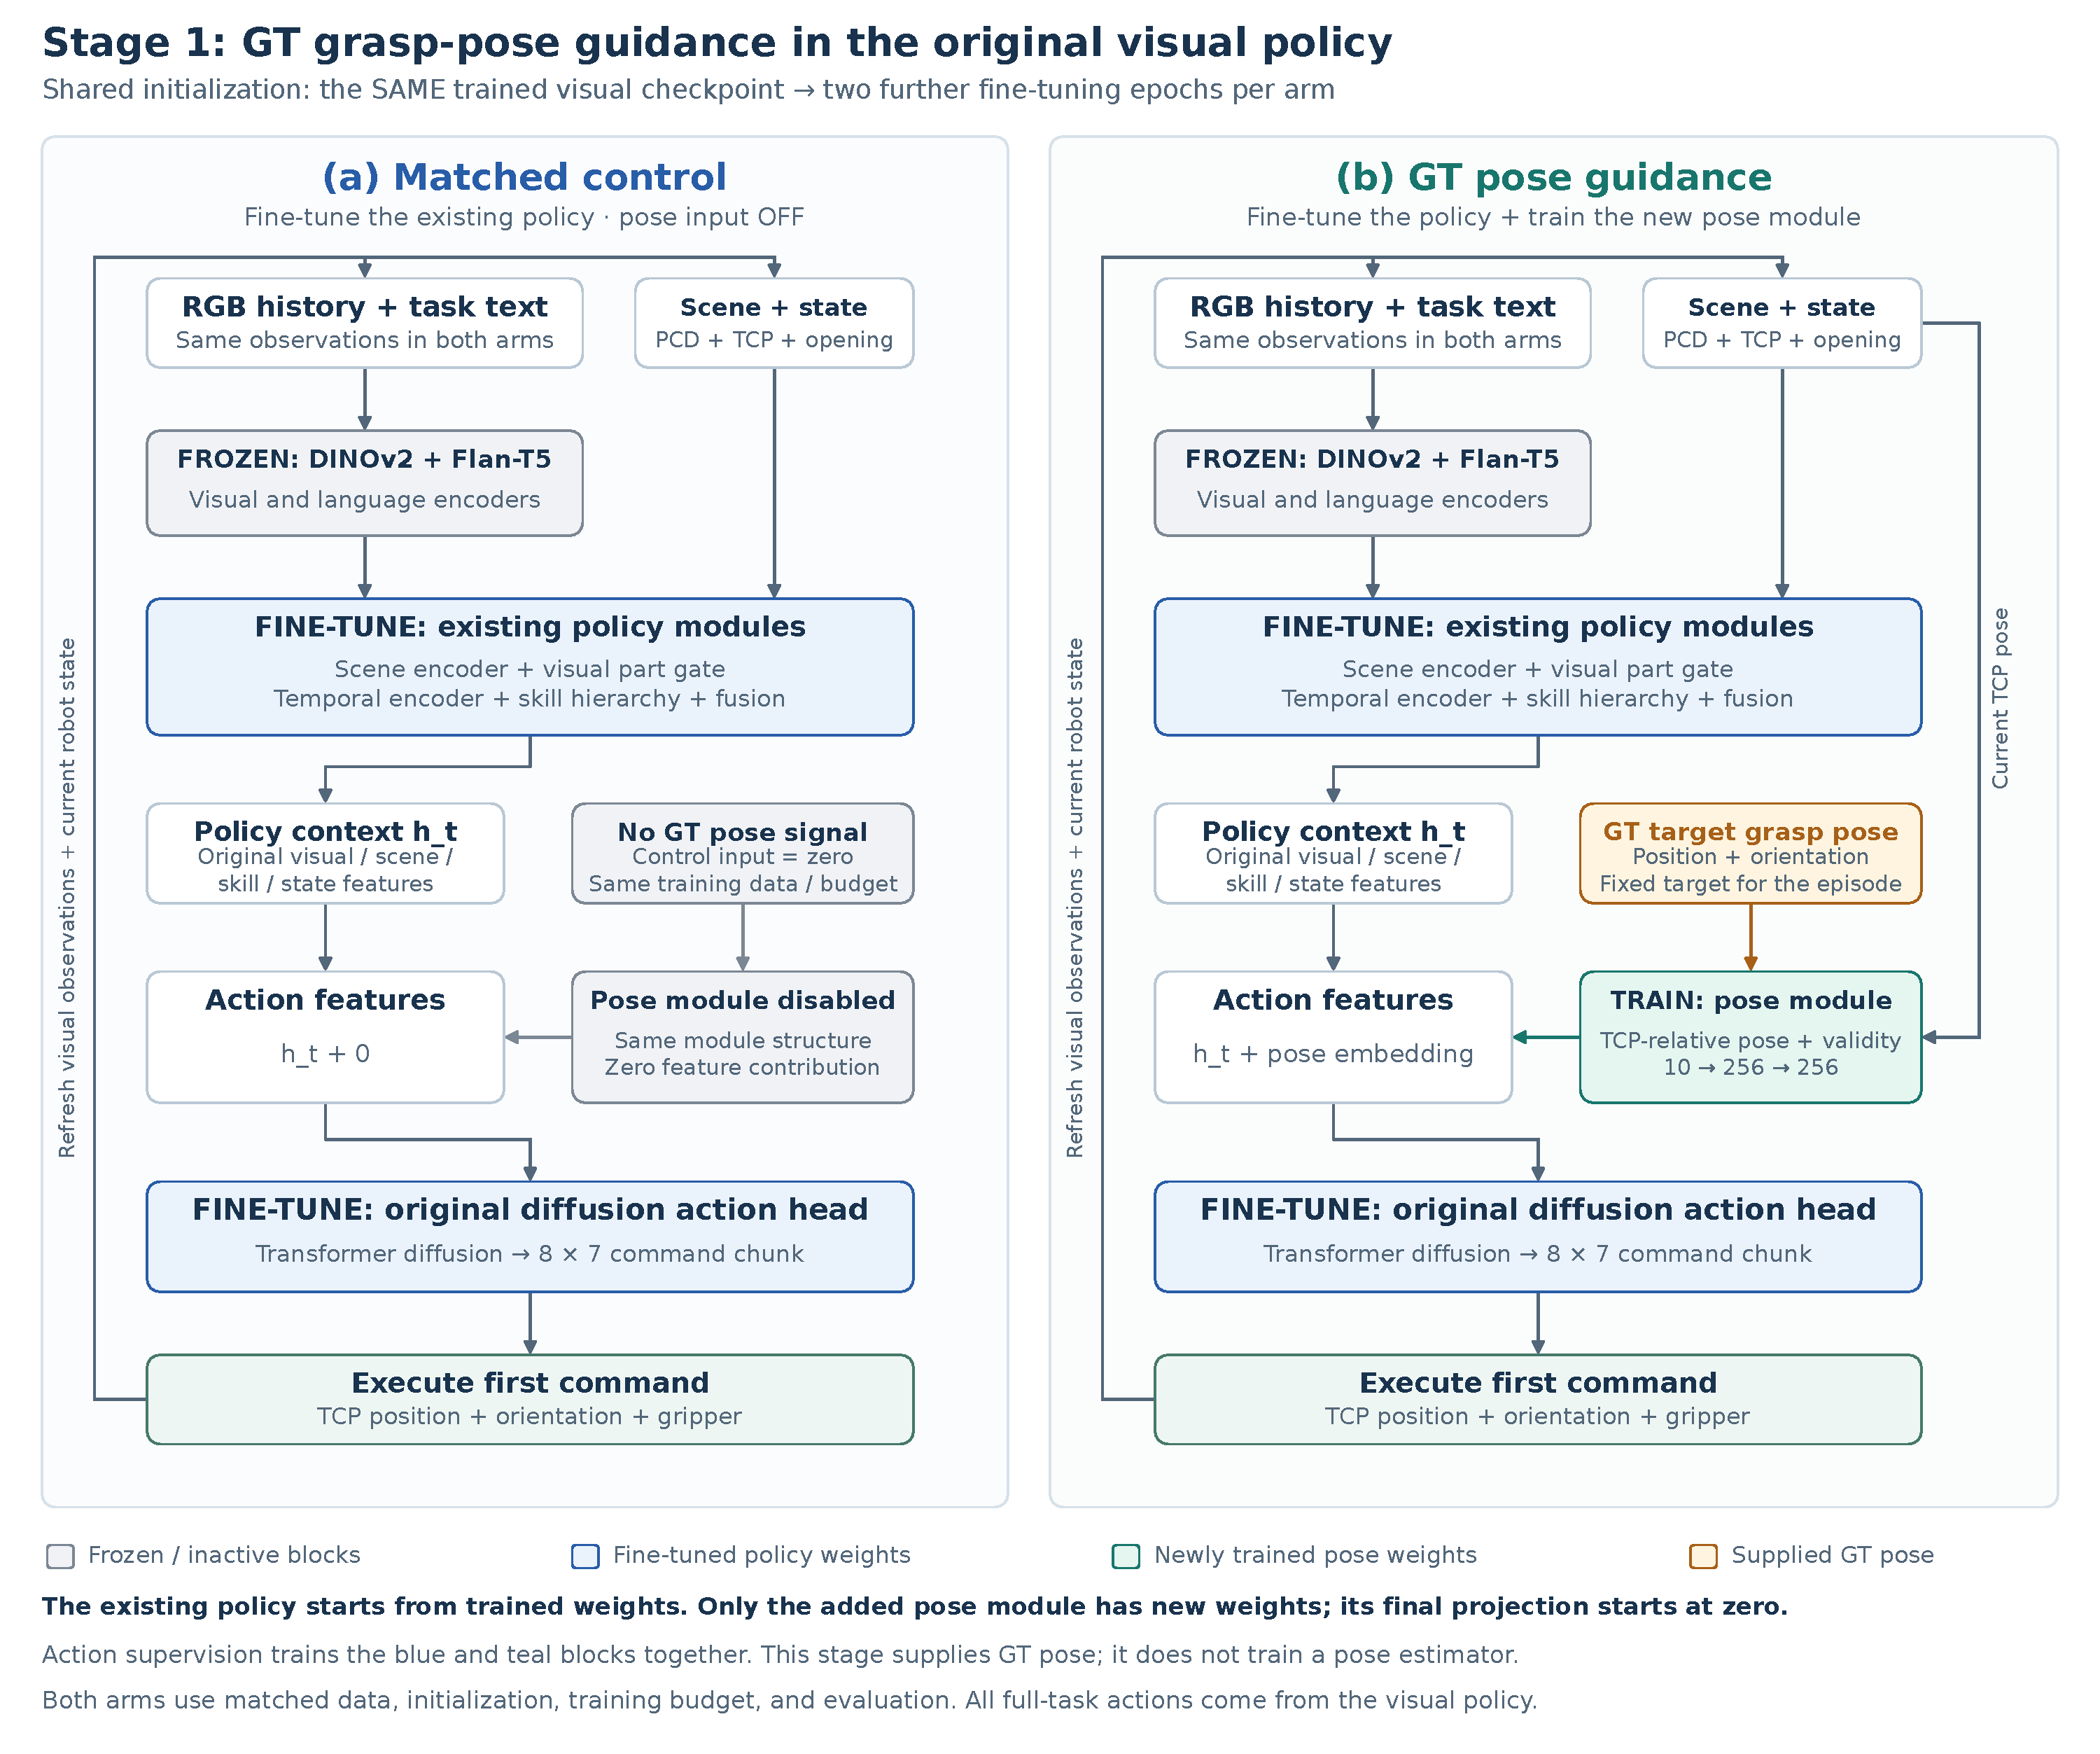
\includegraphics[width=\textwidth]{visual_gt_pose_finetuning.pdf}
  \caption{Matched fine-tuning setup for supplied GT grasp-pose guidance in the
  original visual policy. Both arms initialize shared policy weights from the
  same previously trained checkpoint and retain RGB, scene point clouds,
  language, measured TCP pose, and gripper opening. DINOv2 and Flan-T5 remain
  frozen. Existing scene, grounding, temporal, hierarchy, fusion, and diffusion
  action-head parameters are fine-tuned for two additional epochs in both arms.
  In the GT arm, a newly initialized MLP embeds the target pose relative to the
  current TCP; its contribution is added to the original action features before
  the unchanged diffusion action-head architecture predicts commands. The
  control disables this contribution. A zero-initialized final projection makes
  both arms initially reproduce the old policy. The pose module and existing
  trainable policy parameters learn together from action supervision. GT pose is
  supplied throughout this first-stage oracle experiment; a learned pose
  estimator is reserved for a later stage. All task actions are policy generated.}
  \label{fig:visual-gt-pose-finetuning}
\end{figure*}
